\documentclass[11pt]{beamer}
\usetheme{Warsaw}
\usepackage[utf8]{inputenc}
\usepackage[english]{babel}
\usepackage{amsmath}
\usepackage{amsfonts}
\usepackage{amssymb}
\usepackage{graphicx}
\author{inż. Piotr Zdunek\\
dr inż. Grzegorz Kasprowicz}
\title{High speed multichannel camera with 10 Gbps interface}
%\titlegraphic{    
%                    
%                     
\includegraphics[width=1.8cm,keepaspectratio]{pic/logoEiTI.png}\hspace*{1,5cm}~
%                     
\includegraphics[width=1.8cm,keepaspectratio]{pw-logo.jpg} \hspace*{1,5cm}~
%                     
\includegraphics[width=1.8cm,keepaspectratio]{pic/logo_ise.png} 
%                     
%                     }
%\setbeamercovered{transparent} 
%\setbeamertemplate{navigation symbols}{} 
\logo{               
\includegraphics[width=1cm,keepaspectratio]{pic/logoEiTI.png}\hspace*{0,5cm}
                     
\includegraphics[width=1cm,keepaspectratio]{pw-logo.jpg} \hspace*{0,5cm}
                     
\includegraphics[width=1cm,keepaspectratio]{pic/logo_ise.png} \hspace*{0,5cm}
                     } 
\institute{Warsaw University of Technology\\
Faculty of Electronics and Information Technology\\
Institute of Electronic Systems \\ 
Photonics and Web Engineering Group} 
%\date{} 
\subject{Master Thesis} 
%\setbeamercovered{transparent} 
%\setbeamertemplate{navigation symbols}{} 
%\logo{} 
%\institute{} 
%\date{} 
%\subject{} 
\begin{document}

\begin{frame}
\titlepage
\end{frame}

\begin{frame}
\tableofcontents
\end{frame}

\section{Introduction}
    \begin{frame}{Typical camera overview}
        \begin{minipage}[t]{0.48\linewidth}
            Typical camera mainly consists of:
            \begin{itemize}
                \item optics
                \item shutter
                \item electronics
                \item shutter release
                \item sensor
                \item display
            \end{itemize}
        \end{minipage}\hfill
        \begin{minipage}[t]{0.48\linewidth}
            \begin{figure}[H]
	            \centering
	            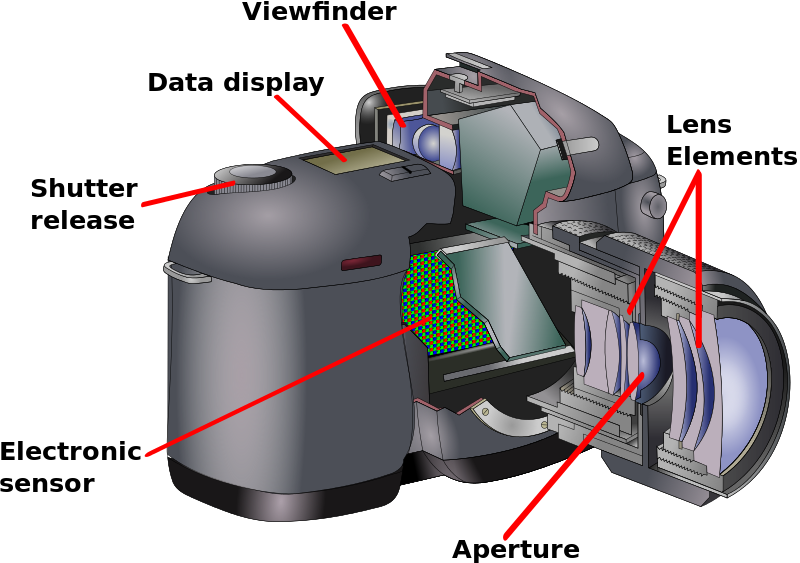
\includegraphics[width=5cm]{pic/camera.png}
	            \caption{Example of camera system}
            \end{figure}
        \end{minipage}
    
    \end{frame}
    
    \begin{frame}{Scientific camera overview}
        \begin{minipage}[t]{0.48\linewidth}
            Scientific camera adds:
            \begin{itemize}
                \item multichannel operation
                \item high speed interface
                \item sophisticated sensor
                \item remote control
                \item no display :(
            \end{itemize}
        \end{minipage}\hfill
        \begin{minipage}[t]{0.48\linewidth}
            \begin{figure}[H]
	            \centering
	            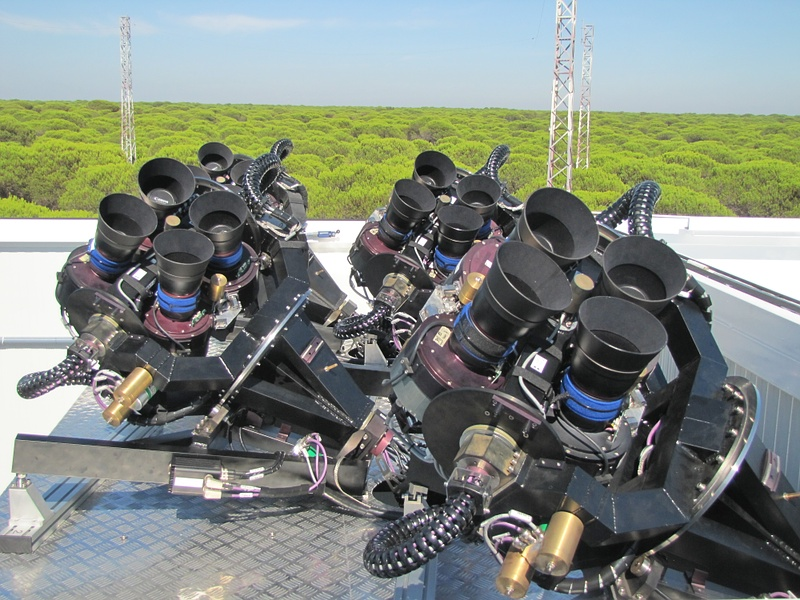
\includegraphics[width=5cm]{pic/camera_pi.jpg}
	            \caption{Pi of the sky camera system}
            \end{figure}
        \end{minipage}
    
        \end{frame}

    \begin{frame}{Genesis}
        \begin{itemize}
            \item there is no open framework for camera design
            \item all designs are custom
            \item long and tedious development
            \item solution?
        \end{itemize}
    
    \end{frame}
    
    \begin{frame}{Goal of the master thesis}
        The goal of my thesis is to design a firmware for a scientific camera with the following                 requirements:
        \begin{itemize}
            \item high processing performance - for support of high resolutions
            \item ease of adding a support for a different sensor
            \item high speed communication - to send high amounts of data live
            \item multichannel operation - astronomical as well as medical applications require it
        \end{itemize}
    \end{frame}
    
\section{Concept of realization}
    \begin{frame}{Concept of realization}

            \begin{figure}[H]
	            \centering
	            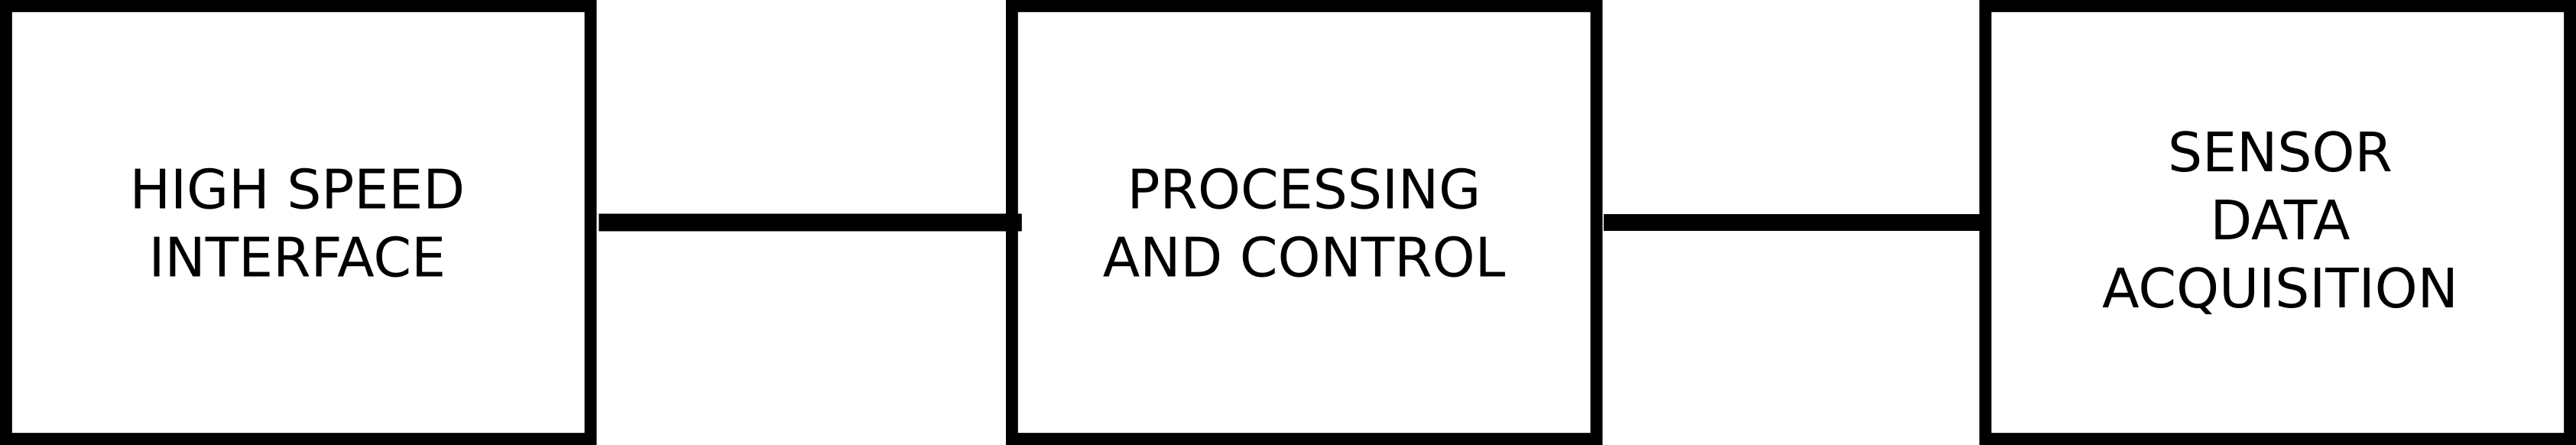
\includegraphics[width=10cm]{pic/camera_system_overview.png}
	            \caption{High speed multichannel camera block diagram}
            \end{figure}
     \end{frame}
     
     \begin{frame}{Concept of realization}

            \begin{figure}[H]
	            \centering
	            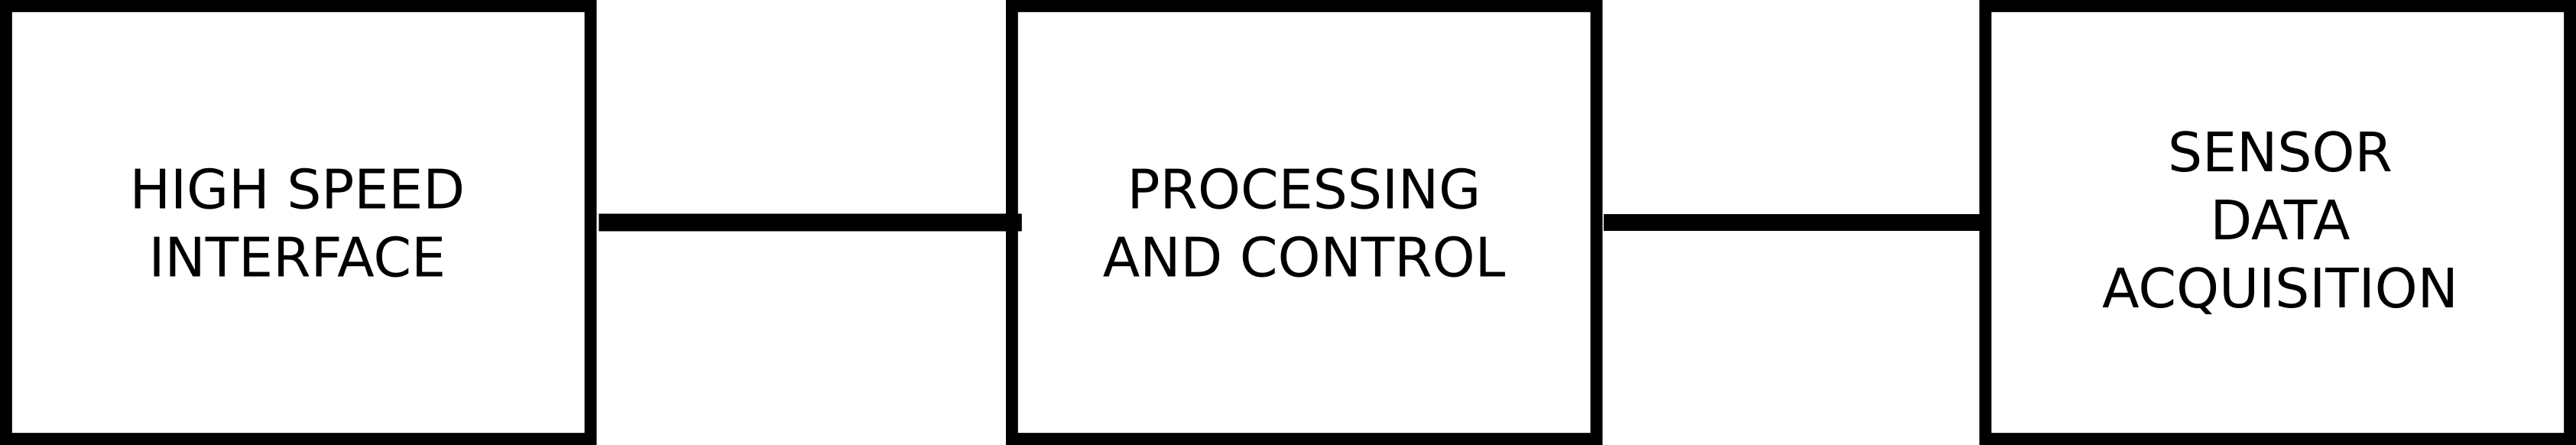
\includegraphics[width=10cm]{pic/camera_system_overview.png}
	            \caption{High speed multichannel camera block diagram}
            \end{figure}
     \end{frame}
     
     
\section{Realization}
    \begin{frame}{dummy}

    \end{frame}
    

\section{Status of development}
    \begin{frame}{dummy}

    \end{frame}
    
\section{Further development}
    \begin{frame}{dummy}

    \end{frame}
    
\section{Summary}
    \begin{frame}{dummy}

    \end{frame}
    
\end{document}}